% !TeX encoding = UTF-8
% 此文件从2023.02开始

%
\chapter{史瓦西时空}\label{chsch}

史瓦西(Karl Schwarzschild,1873.10.9--1916.5.11)解是爱因斯坦引力场方程的第一个精确解.
在一战期间,史瓦西在德国东部战线服役,因患病(天疱疮)返回后方治疗;
他于1916年1月初(爱因斯坦于1915.11.25发现爱氏场方程)给出了这个解.
直到现在,这个解仍是广义相对论中最为重要的解(虽然克尔解更贴近自然界,
但克尔解比史瓦西解复杂太多),此解具有极为广泛的应用.



\section{定态、静态、球对称空间}

\begin{definition}\label{chsch:def_stationary}
    若四维闵氏流形$(M,g)$上存在类时Killing切矢量场$(\frac{\partial }{\partial x^0} )^a
    =(\frac{\partial }{\partial t} )^a$;
    则称流形$M$是{\heiti 定态的}(stationary),$g_{ab}$称为定态度规.
\end{definition}

\begin{definition}\label{chsch:def_static}
    若四维闵氏流形$(M,g)$是定态的,其上存在ADM分解(见\S\ref{chsm:sec_ADM}),
    并且类时Killing切矢量场$(\frac{\partial }{\partial t} )^a$正交于分解后的
    类空超曲面(定义见\ref{chsm:def_hypersurface-orthogonal});
    则称$M$是{\heiti 静态的}(static),$g_{ab}$称为静态度规.
\end{definition}


若$M$是定态的,根据\pageref{chrg:thm_killing-partial-x1}页定理\ref{chrg:thm_killing-partial-x1}可知:
存在局部适配坐标系$(U;x^\mu)$,我们令Killing矢量场$\xi^a |_U = (\frac{\partial }{\partial x^0} )^a
=(\frac{\partial }{\partial t} )^a$,
那么必然有$\Lie_{\xi} g_{\mu\nu}= \frac{\partial g_{\mu\nu}}{\partial t}=0$.
这就是说存在适配坐标系$(U;x^\mu)$使得度规的所有分量都不含有参数$x^0\equiv t$.
需要指出的是并不是任意给定一个局部坐标系,度规所有分量$g_{\mu\nu}$便不含有某个坐标;
只要存在一个这样的局部坐标系即可.
此处,我们要求存在Killing场$\xi^a$最主要的目的就是令度规分量不含参数$t$.

%比如站在地球表面不动的你会发现地球的引力场是不随时间改变的.

进一步假设$M$是静态的,我们在分解后的类空超曲面$\Sigma_t$上选择三个正交的局部坐标$(\Sigma_t, x^i)$.
因Killing场$\xi^a =(\frac{\partial }{\partial t} )^a$正交于$\Sigma_t$,故必有
\begin{equation}
    g_{0i} = g_{ab}\left(\frac{\partial }{\partial t} \right)^a 
    \left(\frac{\partial }{\partial x^i} \right)^b    =0, \qquad i=1,2,3
\end{equation}

对于静态时空$M$,我们再假设它的类空超曲面族$\{\Sigma_t\}$是球对称的,
根据第\pageref{chhss:tab-msss}页表\ref{chhss:tab-msss}可知
此时的时空线元可表示为(即式\eqref{chhss_eqn_g-st-sphere}):
\begin{equation}\label{chsch:eqn_tmpSchw}
    \mathrm{d} s^2=  g_{00}(r) \mathrm{d} t^2+g_{r r}(r) \mathrm{d} r^2 
    +r^2\left\{\mathrm{d} \theta^2+\sin ^2 \theta \mathrm{d} \phi^2\right\} .
\end{equation}
上式已令$f(r)=r^2$,这相当于把式\eqref{chhss_eqn_g-st-sphere}作了一个变量代换.即,令
\begin{align*}
    r'^2 = f(r);\qquad \text{反解出} \, r=f^{-1}(r'^2) \text{,再带回去,并省略撇号}
\end{align*}

式\eqref{chsch:eqn_tmpSchw}便是静态、球对称时空$(M,g)$度规线元的形式;
这个时空的等距群$I(M)=\mathbb{R}\times SO(3)$,
其中$\mathbb{R}$是指实数加法群,参见例\ref{chlg:exam_Rplus}.



\paragraph{定态场的四加速度}

设定态场中的Killing矢量场$\xi^a$是{\kaishu 类时}的,其积分曲线自然是一个观测者,
但$\xi^a$未必是归一的;令其归一化切矢量为$Z^a$,易得:$\xi^a=\sqrt{-g_{00}}Z^a$.
此时$Z^a$便是一个定态观测者,它的积分曲线与$\xi^a$的积分曲线重合,但参数化不同.
由前面不分析不难知道$g_{00}$是不含时的,
也就是$\nabla_\xi g_{00}=\nabla_{\frac{\partial}{\partial t}}g_{00}
=\frac{\partial g_{00}}{\partial t}=0$;
由此不难求得定态观测者$Z^a$的四加速度:
\begin{align}
    A_a =& \nabla_Z Z_a = \frac{1}{\sqrt{-g_{00}}} \nabla_\xi \frac{\xi_a}{\sqrt{-g_{00}}}
    = \frac{1}{-g_{00}} \xi^b\nabla_b \xi_a  \xlongequal{\ref{chrg:eqn_killing-2}}
    \frac{1}{g_{00}} \xi^b\nabla_a \xi_b \notag \\
    =& \frac{1}{2 g_{00}} \nabla_a \left(\xi^b \xi_b\right)
    =\frac{1}{-2 g_{00}} \nabla_a \left(- g_{00} \right)
    =\nabla_a \left(\ln \sqrt{- g_{00}} \right) . \label{chsch:eqn_A-stationary}
\end{align}

我们已知$Z^a A_a=0$,由命题\ref{chnull:thm_tl-sl}可知$A_a$必是类空的.



\section{史瓦西真空解}
略微更改一下式\eqref{chsch:eqn_tmpSchw}中的记号,
在局部坐标系$\{t,r,\theta,\phi\}$上度规线元为:
\begin{equation}\label{chsch:eqn_Schw-metric-raw}
    {\rm d}s^2 = -e^{2 \alpha(r)} {\rm d}t^2 + e^{2 \beta(r)} {\rm d}r^2
      + r^2 {\rm d}\theta^2 + r^2 \sin^2\theta {\rm d}\phi^2 .
\end{equation}
如果读者不了解对称空间等知识,那么可以直接假设度规线元为上式,
而去关注此时会有怎样的爱因斯坦引力场方程解!
其实,史瓦西最早就是假设线元写成上述形式,
然后把它带入真空爱氏方程求解的,可参见\parencite{schwarzschild-1999}.



由式\eqref{chsch:eqn_Schw-metric-raw}求得非零克氏符为
(其中“$'$”表示对“$r$”求导):
\begin{subequations}\label{chsch:eqn_Schw-ksf-raw}
    \begin{align}
       &\Gamma^0_{01}= \Gamma^0_{10} = \alpha',\quad
        \Gamma^1_{00}= \alpha' e^{2(\alpha-\beta)}, \quad
        \Gamma^1_{11}= \beta', \\
       &\Gamma^1_{22}= -r e^{-2\beta}, \quad
       \Gamma^1_{33}= -r \sin^2\theta e^{-2\beta}, \quad
        \Gamma^2_{12}=\Gamma^2_{21}= \frac{1}{r}, \\
       &\Gamma^2_{33}=-\sin\theta \cos\theta, \quad
       \Gamma^3_{13}=\Gamma^3_{31}=\frac{1}{r}, \quad
        \Gamma^3_{23}=\Gamma^3_{32}=\cot\theta .
    \end{align}
\end{subequations}
由上式求出非零黎曼曲率是
\setlength{\mathindent}{0em}
\begin{subequations}\label{chsch:eqn_Schw-riemann-raw}
\begin{align}
R_{0101} =& e^{2 \alpha } \left(\alpha'^2- \alpha'\beta'+\alpha''\right), \quad
R_{0202} = e^{2 \alpha -2 \beta } r \alpha ', \quad
R_{1212} = r \beta ', \\
R_{0303} =& e^{2 \alpha -2 \beta } r \alpha ' \sin ^2\theta  , \
R_{1313} = r \beta ' \sin ^2\theta  ,\
R_{2323} = \left(1-e^{-2 \beta}\right) r^2 \sin ^2\theta.
\end{align}
\end{subequations}\setlength{\mathindent}{2em}
由上式求出非零Ricci曲率是
\begin{subequations}\label{chsch:eqn_Schw-ricci-raw}
\begin{align}
    R_{00} =&  e^{2(\alpha-\beta)} ( \alpha'' - \alpha'\beta'
      +\alpha'^2 +2 r^{-1} \alpha' ) , \\
    R_{11} =& - \alpha'' + \alpha'\beta' -\alpha'^2  +2 r^{-1} \beta'  , \\
    R_{22} =& 1 - e^{-2\beta} \bigl(1+ r(\alpha'-\beta')\bigr), \\
    R_{33} =& \Bigl(1 - e^{-2\beta} \bigl(1+ r(\alpha'-\beta')\bigr)\Bigr)\sin^2\theta .
\end{align}
\end{subequations}
可由\eqref{chfd:eqn_Einstein-B-form}得到真空爱氏场方程:$R_{ab}=0$;
将上式带入,有
\begin{align}
    - \alpha'' + \alpha'\beta' -\alpha'^2 -2 r^{-1} \alpha' =& 0 , \label{chsch:eqn_tmp-ab1} \\
    - \alpha'' + \alpha'\beta' -\alpha'^2 +2 r^{-1} \beta'  =& 0 , \label{chsch:eqn_tmp-ab2} \\
    1 - e^{-2\beta} \bigl(1+ r(\alpha'-\beta')\bigr) =& 0 . \label{chsch:eqn_tmp-ab3} 
\end{align}
由式\eqref{chsch:eqn_tmp-ab1}、\eqref{chsch:eqn_tmp-ab2}可得
\begin{equation}\label{chsch:eqn_apb=0}
    \alpha'(r) + \beta'(r)=0 \quad \Rightarrow \quad
    \alpha(r)= -\beta(r) + C_0 .
\end{equation}
将上式带入式\eqref{chsch:eqn_tmp-ab3},有
\begin{equation}
    e^{2\beta} = 1-2r \beta'(r) .
\end{equation}
容易得到上述常微分方程组的解
\begin{equation}\label{chsch:eqn_ab0}
    e^{2\beta}  = \left(1+\frac{C_1}{r}\right)^{-1} , \quad \text{及} \quad 
    e^{2\alpha} = e^{2C_0} \left(1+\frac{C_1}{r}\right) .
\end{equation}
我们定义一个新的时间$t'\equiv e^{C_0} t$(注$C_0$是常数),
则有$\frac{\partial }{\partial t'}=e^{-C_0}\frac{\partial }{\partial t}$;
可见$(\frac{\partial }{\partial t'})^a$仍是Killing矢量场.
因此,我们可以选取$t'$当成新的{\kaishu 时间},并省略撇号.
此时,爱氏方程解为
\begin{equation}
    {\rm d}s^2 = -\left(1+\frac{C_1}{r}\right) {\rm d}t^2
    + \left(1+\frac{C_1}{r}\right)^{-1} {\rm d}r^2
    + r^2 {\rm d}\Omega.
\end{equation}
其中
\begin{equation}\label{chsch:eqn_dOmega}
    {\rm d}\Omega\equiv({\rm d}\theta)^2 + (\sin\theta {\rm d}\phi)^2 .
\end{equation}
我们(可能只是笔者自己?)并不是很准确地知道爱因斯坦引力场方程的边界条件,
只能泛泛地提一些要求;比如当$r\to \infty$时,引力场变成弱场,
非线性爱氏方程趋于线性爱氏方程\eqref{chle:eqn_Einstein-1},
度规场$g_{ab}$趋于式\eqref{chle:eqn_g-eta+h},即平直的洛伦兹度规附加一个线性项.
此时,上式变为
\begin{equation}
    {\rm d}s^2(r\to \infty) = -\frac{C_1}{r}\left( {\rm d}t^2 +{\rm d}r^2 \right)  
    + \left\{{-\rm d}t^2 + {\rm d}r^2+r^2 {\rm d}\Omega \right\}.
\end{equation}
很明显,上式中花括号内的部分“$\{{-\rm d}t^2 + {\rm d}r^2+r^2 {\rm d}\Omega \}$”是平直的洛伦兹度规.
对比弱场下的式\eqref{chle:eqn_hab}和
式\eqref{chsr:eqn_Newton-gravity-potential}($\Phi=-\frac{GM}{r}$)可得:$C_1=-2GM/c^2$.

进而有国际单位制下的{\heiti 史瓦西线元}:
\begin{equation}\label{chsch:eqn_Schw-metric}
    {\rm d}s^2 = - \left(1-\frac{2G M}{c^2 r}\right) (c{\rm d}t)^2
    + \left(1-\frac{2G M}{c^2 r}\right)^{-1} ({\rm d}r)^2
    + r^2 {\rm d}\Omega.
\end{equation}
上式中的$\{t,r,\theta,\phi\}$称为{\heiti 史瓦西坐标}.
定义{\heiti 史瓦西半径}为:
\begin{equation}\label{chsch:eqn_Schw-radius}
    R_s \equiv \frac{2G M}{c^2} .
\end{equation}
之后,我们将采用自然单位制,即令$G=1=c$.
常见天体的史瓦西半径:
太阳$R_s\approx 2.95 \si{km}$;
地球$R_s\approx 8.87 \si{mm}$;
月亮$R_s\approx 0.109 \si{mm}$;
木星$R_s\approx 2.82 \si{m}$.


不难发现当$r=0$、$r=R_s$时,
史瓦西度规\eqref{chsch:eqn_Schw-metric}是奇异的(出现无穷大);
后面我们会指出$r=R_s$是坐标奇性(假的),$r=0$是真奇性.
我们姑且假定史瓦西真空解\eqref{chsch:eqn_Schw-metric}只在$r>2M$时是适用的;
可见太阳的史瓦西半径完全在太阳内部,故这种限制完全不影响史瓦西真空解的使用.

%史瓦西度规\eqref{chsch:eqn_Schw-metric}有以下几点属性:
%(1) 渐进平坦.当$r\to \infty$时,它趋近于平直的洛伦兹度规,弯曲时空趋于平直的闵氏时空.
%这符合物理认知,比如在不考虑有其他星体前提下,离太阳无限远处肯定是没有引力的平直时空.


\begin{example}
    地球的重力加速度.
\end{example}

式\eqref{chsch:eqn_A-stationary}给出的四加速度便对应的牛顿力学中的天体重力加速度.
我们先求出史瓦西解下的四加速(类空矢量),再求出其长度.
\begin{align}
    A_a = & %\frac{1}{-2 g_{00}} \nabla_a \left(- g_{00} \right) =
    \frac{1}{2} \left(1-\frac{2 M}{ r}\right)^{-1} {\rm d}_a \left(1-\frac{2 M}{ r}\right)
    =\left(1-\frac{2 M}{ r}\right)^{-1} \frac{ M}{ r^2}({\rm d}r)_a . \\
    |A|=& \sqrt{g^{ab}A_a A_b} = \left(1-\frac{2G M}{c^2 r}\right)^{-1/2}
    \frac{G M}{ r^2}. \label{chsch:eqn_A-module}
\end{align}
式\eqref{chsch:eqn_A-module}已用国际制表示.
将地球数据带入后,其值约等于$9.8 \si{m/s^2}$.
\qed


为了方便使用,我们给出史瓦西时空的非零克氏符:
\begin{equation}\label{chsch:eqn_Schw-Christoffel}
	\begin{aligned}
		&\Gamma^0_{01}= \Gamma^0_{10} = \frac{M}{r^2-2 M r},\
		\Gamma^1_{00}= \frac{M (r-2 M)}{r^3}, \
		\Gamma^1_{11}= \frac{M}{2 M r-r^2}, \\
		&\Gamma^1_{22}= 2 M-r, \quad
		\Gamma^1_{33}= (2 M-r) \sin ^2\theta  , \quad
		\Gamma^2_{12}=\Gamma^2_{21}= \frac{1}{r}, \\
		&\Gamma^2_{33}=-\sin\theta \cos\theta, \quad
		\Gamma^3_{13}=\Gamma^3_{31}=\frac{1}{r}, \quad
		\Gamma^3_{23}=\Gamma^3_{32}=\cot\theta .
	\end{aligned}
\end{equation}
以及非零的黎曼曲率:
\begin{equation}\label{chsch:eqn_Schw-Riemann}
	\begin{aligned}
		R_{0101}=&-\frac{2 M}{r^3},\, R_{0202}=\frac{M(r-2M)}{r^2},\, R_{0303}=\frac{M(r-2M)}{r^2} \sin ^2 \theta, \\ 
		R_{1212}=&\frac{-M}{r-2M}, \ R_{1313}=\frac{-M\sin ^2 \theta}{r-2M}, \ R_{2323}=2 M r \sin ^2 \theta .
	\end{aligned}
\end{equation}



\section{测地偏离与潮汐力}\label{chsch:sec_GDTF}
根据\S\ref{chfd:sec_Fundamental-Postulate}中的假设\fbox{甲}(引力几何化)和等效原理
(或\S\ref{chfd:sec_sr2gr}中的最小替换法则)可知在爱因斯坦的引力论中自由质点沿时空测地线运动.
我们将仅根据上述假设给出广义相对论中的测地偏离运动,它与牛顿力学中的潮汐力相对应.
将此节写在这里的主要原因是想使用一下史瓦西度规中的黎曼曲率\eqref{chsch:eqn_Schw-Riemann}.

为简单起见,我们只考虑地球的潮汐力,不考虑月亮、太阳引起的潮汐力.
设有地球表面有两个质点(分别称为A和B),高度不同(但相距非常近),两者连线的延长线通过地心.
A、B都作测地运动,它们的测地线参数方程分别是$\gamma(\tau)$、$\gamma(\tau+\Delta\tau)$;
两者之间的距离$J^a$是一个四维矢量.
回忆\S\ref{chgd:sec_Jacobi}中的Jacobi方程\eqref{chgd:eqn_Jacobi}正是描述两条测地线间距离矢量
随测地线线长(类时线线长即为固有时$\tau$)变化的方程式(下式中$Z^c$是$\gamma(\tau)$的切线切矢量)
\begin{equation}
	\nabla_{\frac{\partial}{\partial \tau}} \nabla_{\frac{\partial}{\partial \tau}}{J}^a =
	R^{a}_{\hphantom{a} bcd} {Z}^c{J}^d {Z}^b. 
\end{equation}
我们选沿$\gamma(\tau)$的一个四标架场,并令$Z^a$为第零标架.


由\eqref{chsch:eqn_Schw-Riemann}可得
\begin{align}
		R^1_{\phantom{1}001}=&\frac{2 M}{r^3}\left(1-\frac{2M}{r}\right)\approx \frac{2 M}{r^3}
		=\frac{2 G^3 M}{c^6 r^3} ,\\
		R^2_{\phantom{1}002}=&\frac{M(r-2M)}{-r^4}\approx -\frac{M}{r^3}=-\frac{G^3 M}{c^6 r^3},\\ 
		R^3_{\phantom{1}003}=&\frac{M(r-2M)}{-r^4}\approx -\frac{M}{r^3}=-\frac{G^3 M}{c^6 r^3}.
\end{align}
对比式\eqref{chsr:eqn_Ri00k}可知:除了系数$G$、$c$外,两者相同.注意上面三式中的“$1$”分量对应“$z$”.
我们把上面三式带入\eqref{chsr:eqn_TF-R},并恢复有量纲情形,有
\begin{align*}
	f^i_T = &  m R_{\hphantom{i}00k}^i x^k  \quad \Rightarrow \\
	\frac{\boldsymbol{f}_T}{c^4 G^{-1}} = & m R^3_{\phantom{3}003} \frac{x}{c^{-2}G}\boldsymbol{e}_x
	+m R^2_{\phantom{2}002} \frac{y}{c^{-2}G}\boldsymbol{e}_y
	+m R^1_{\phantom{1}001} \frac{z}{c^{-2}G}\boldsymbol{e}_z \quad \Rightarrow  \\
	\boldsymbol{f}_T = & \frac{G M m}{r^3} \left( -x \boldsymbol{e}_x -y \boldsymbol{e}_y+ 2z \boldsymbol{e}_z \right) .
\end{align*}
最终得到公式与式\eqref{chsr:eqn_Tidal-Force}相同.



\section{Reissner--Nordstr\"om度规}
史瓦西解是静态球对称天体的外部真空(vaccum)时空.
有些天体自身携带一些电荷,在天体外部存在电磁场.
我们把没有实物粒子、只有电磁场的时空称为{\heiti 电磁真空}(electrovaccum).
下面寻找电磁真空下的爱氏方程解.

时空仍是球对称、静态的,故线元仍为式\eqref{chsch:eqn_Schw-metric-raw}.
此时电磁场也是球对称、静态的,故规范势$A_\mu$只是$r$的函数,
不含有$t$、$\theta$、$\phi$;且$A_\theta=0=A_\phi$.
当我们规范势描述电磁场时,是存在规范变换自由度的;
故,通过规范变换可令$A_r=0$;但这些不同的规范势对应同一个电磁张量$F_{\mu\nu}$.
因此,只剩下$A_t(r)$项,将$A_t(r)$简记为$A(r)$.

由电磁场张量\eqref{chlh:eqn_Fab}可得史瓦西坐标$\{t,r,\theta,\phi\}$下的非零分量:
\begin{equation}
    F_{10}=-F_{01}= \frac{{\rm d}A(r)}{{\rm d}r} = A' . \qquad
    F^{10}=-F^{01}=-e^{-2\alpha-2\beta}A' .
\end{equation}
容易算出$\sqrt{-g}=e^{\alpha+\beta}r^2 \sin^2\theta$.
需用麦氏方程组\eqref{chlh:eqn_Maxwell-1}
($\partial_\mu \left(F^{\nu\mu} \sqrt{-g} \right) = 0$)来求解;
不难得到非恒零方程为($\nu=0$):
\begin{equation}
    \frac{{\rm d}}{{\rm d}r} \left( e^{-\alpha-\beta} r^2 A' \sin^2\theta \right) =0.
\end{equation}
积分之,有
\begin{equation}
    F_{10}= A' = \frac{Q}{4\pi r^2} e^{\alpha+\beta},\quad
    F_{ab}=-\frac{Q}{4\pi r^2} ({\rm d}t)_a \wedge ({\rm d} r)_b .
\end{equation}
其中$Q$是积分常数.
显然还没有求解完毕;剩余部分需要解爱氏场方程.

借助符号演算软件,由式\eqref{chlh:eqn_EM-tensor-down}可得:
\begin{equation}
\begin{aligned}
    T_{00}=& \frac{1}{2} e^{-2 \beta } (F_{10})^2,\qquad\quad
    T_{11}= -\frac{1}{2} e^{-2 \alpha }(F_{10})^2, \\
    T_{22}=& \frac{r^2}{2} e^{-2 (\alpha +\beta )}  (F_{10})^2,\quad
    T_{33}= \frac{r^2}{2} e^{-2 (\alpha +\beta )}  (F_{10})^2 \sin ^2\theta   .
\end{aligned}
\end{equation}
将上式带入电磁真空爱氏场方程($G_{\mu\nu}=8\pi T_{\mu\nu}$);
注意到电磁场能动张量是无迹的(请读者自行验证),有
\begin{align}
    &  e^{2(\alpha-\beta)} ( \alpha'' - \alpha'\beta'
    +\alpha'^2 +2 r^{-1} \alpha' ) = 4\pi e^{-2 \beta } (F_{10})^2, \\
    & - \alpha'' + \alpha'\beta' -\alpha'^2  +2 r^{-1} \beta'  
    =-4\pi  e^{-2 \alpha }(F_{10})^2, \\
    & 1 - e^{-2\beta} \bigl(1+ r(\alpha'-\beta')\bigr)
    =4\pi r^2 e^{-2 (\alpha +\beta )}  (F_{10})^2  \label{chsch:eqn_R22=T22}.
\end{align}
由前两式可得$\alpha'+\beta'=0$(与式\eqref{chsch:eqn_apb=0}相同),
那么由此得到解也与真空史瓦西情形相同;
再由式\eqref{chsch:eqn_R22=T22}得
\begin{align}
1 - e^{-2\beta} \bigl(1- 2r\beta'\bigr)= \frac{Q^2}{4\pi r^2} 
\quad \Rightarrow \quad
e^{2\beta}  = \left(1-\frac{2M}{r}+\frac{Q^2 }{4\pi r^2}\right)^{-1} .
\end{align}
已选积分常数$M$与史瓦西度规相同.自然有(已选新$t$与史瓦西度规相同)
\begin{equation}
    e^{2\alpha} =1-\frac{2 M}{ r}+ \frac{Q^2 }{4\pi r^2} .
\end{equation}



最终,国际单位制下的{\bfseries\heiti Reissner--Nordstr\"om线元}(简称{\bfseries\heiti RN线元})为:
\begin{equation}\label{chsch:eqn_RN-metric}
\begin{aligned}
    {\rm d}s^2 =& - \left(1-\frac{2G M}{c^2 r}+ \frac{Q^2 G }{4\pi \epsilon_0 c^4 r^2} \right) (c{\rm d}t)^2
    + ({\rm d}r)^2 \times \\
    &\times \left(1-\frac{2G M}{c^2 r}+\frac{Q^2 G }{4\pi \epsilon_0 c^4 r^2}\right)^{-1}  
    + r^2 \left(({\rm d}\theta)^2 + (\sin\theta {\rm d}\phi)^2\right).
\end{aligned}    
\end{equation}


\section{史瓦西测地线}



类时(或类光)测地线$\gamma(\tau)$方程\eqref{chgd:eqn_geodesic-formula}为
\begin{equation}
    \frac{{\rm d}^2 x^\rho(\tau)}{{\rm d}\tau^2} + \Gamma_{\mu\nu}^\rho(\tau)
    \frac{{\rm d}x^\mu(\tau)}{{\rm d} \tau} \frac{{\rm d}x^\nu(\tau)}{{\rm d} \tau} =0.
    \tag{\ref{chgd:eqn_geodesic-formula}}
\end{equation}
对于类时测地线,$\tau$是固有时;
对于类光测地线,$\tau$是一个仿射参数;
$x^\mu(\tau)$是$\gamma(\tau)$在局部坐标系$\{t,r,\theta,\phi\}$的分量参数.

从史瓦西线元\eqref{chsch:eqn_Schw-metric}可以看出它关于$\theta=\pi/2$对称,
即在变换$\theta \to \pi -\theta$下不变.
故我们猜测测地线中的$\theta$可以恒为$\pi/2$.
又因为测地线解是唯一的,故只需验证$\theta=\pi/2$是不是
方程\eqref{chgd:eqn_geodesic-formula}的解即可.
令$\rho=2$,结合式\eqref{chsch:eqn_Schw-Christoffel}有
\begin{equation}
    \frac{{\rm d}^2 \theta}{{\rm d}\tau^2} 
    + \frac{2}{r} \frac{{\rm d}r}{{\rm d} \tau}  \frac{{\rm d}\theta}{{\rm d} \tau} 
    -\sin\theta \cos\theta \left(\frac{{\rm d} \phi}{{\rm d} \tau} \right)^2=0.
\end{equation}
取初始条件为:$\theta(0)=\pi/2$、$\frac{{\rm d}\theta}{{\rm d} \tau}(0)=0$;
上式满足这样初条件的唯一解便是$\theta=\pi/2$.
这便说明了:通过坐标变换可令所有史瓦西测地线中的$\theta=\pi/2$.


我们将根据\pageref{chrg:thm_killing-geodisic}页的定理\ref{chrg:thm_killing-geodisic}定义
几个沿测地线的守恒量;这是此定理在广义相对论中的重要应用.
测地线$\gamma(\tau)$的切线切矢量为$U^a=( \frac{\partial }{\partial \tau} )^a$.
我们将测地线$\gamma(\tau)$在史瓦西坐标中的分量为:$\{t,r,\pi/2,\phi\}$.
史瓦西时空共有四个Killing场,其中一个类时场为$( \frac{\partial }{\partial t} )^a$.
另外三个类空,已在\S\ref{chlg:sec_S2}给出,即二维球面上的三个Killing场\eqref{chlg:eqn_S2-killing}.
定义
\begin{align}
    E\overset{def}{=} & -g_{ab} \left( \frac{\partial }{\partial \tau} \right)^a
    \left( \frac{\partial }{\partial t} \right)^b
    =-g_{00} \frac{{\rm d} t}{{\rm d} \tau}
    = \left(1-\frac{2 M}{ r}\right) \frac{{\rm d} t}{{\rm d} \tau}. \label{chsch:eqn_E-gd} \\
    L\overset{def}{=} & -g_{ab} \left( \frac{\partial }{\partial \tau} \right)^a
    \left( \frac{\partial }{\partial \phi} \right)^b
    =-r^2 \sin^2\theta \frac{{\rm d} \phi}{{\rm d} \tau}
    =-r^2  \frac{{\rm d} \phi}{{\rm d} \tau}. \label{chsch:eqn_L-gd} \\
    L_1 \overset{def}{=} & g_{ab} \left( \frac{\partial }{\partial \tau} \right)^a \xi_1^b
    = r^2 \sin \phi\frac{{\rm d} \theta}{{\rm d} \tau} + r^2 \sin\theta \cos\theta \cos\phi
     \frac{{\rm d} \phi}{{\rm d} \tau}=0.     \label{chsch:eqn_L1-gd} \\
    L_2 \overset{def}{=} & g_{ab} \left( \frac{\partial }{\partial \tau} \right)^a \xi_2^b
    = -r^2 \cos \phi \frac{{\rm d} \theta}{{\rm d} \tau}+ r^2 \sin\theta \cos\theta \sin\phi
    \frac{{\rm d} \phi}{{\rm d} \tau}=0.      \label{chsch:eqn_L2-gd} 
\end{align}

%    \left[ \sin\phi \left(\frac{\partial }{\partial \theta}\right)^b 
%+ \cot\theta \cos\phi \left(\frac{\partial }{\partial \phi}\right)^b \right]
%    \left[-\cos\phi\left(\frac{\partial }{\partial \theta}\right)^b
%+\cot\theta\sin\phi \left(\frac{\partial }{\partial \phi}\right)^b\right] 

上面已把$\theta=\pi/2$带入式\eqref{chsch:eqn_L-gd} -- \eqref{chsch:eqn_L2-gd}, 
发现$L_1$、$L_2$恒为零.守恒量只剩下$E$、$L$,下面将解释它们的物理意义.

单位类时切矢量
\begin{equation}
	Z^a = \left(1-\frac{2M}{r}\right)^{-1/2} \left( \frac{\partial }{\partial t} \right)^a .
\end{equation}
我们先看$E$的含义
\begin{align*}
	E=&-g_{ab} \left( \frac{\partial }{\partial \tau} \right)^a
	\left( \frac{\partial }{\partial t} \right)^b
	=-g_{ab} U^a Z^b \sqrt{1-\frac{2M}{r}} 
	=-g_{ab} P^a Z^b \frac{1}{m}\sqrt{1-\frac{2M}{r}}  \\
	=& E_{\rm local} \times \frac{1}{m} \times \sqrt{1-\frac{2M}{r}}.
\end{align*}
当$r\to \infty$时,$E$的物理意义是单位质量能量.沿测地线$E$是守恒量,但$E_{\rm local}$不是。
可以这样理解此事,$E_{\rm local}$不含引力能,$E$含有引力能。

为看清$L$物理意义,我们先叙述三维空间角动量。
\begin{align*}
	J_a =& \hat{\Omega}_{abc} r^b P^c_{\phi} = \hat{\Omega}_{abc} r (e_1)^b  m U^c_{\phi}
	= mr (Z^e\Omega_{eabc})  \sqrt{1-\frac{2M}{r}} \left( \frac{\partial }{\partial r} \right)^b  
	\left( \frac{\partial }{\partial \phi} \right)^c \frac{{\rm d}\phi }{{\rm d} \tau}  \\
	=&-L m r^{-1}  \left( \frac{\partial }{\partial t} \right)^e \Omega_{eabc}
	\left( \frac{\partial }{\partial r} \right)^b \left( \frac{\partial }{\partial \phi} \right)^c \\
	=& -L m r^{-1}  \left( \frac{\partial }{\partial t} \right)^e r^2 ({\rm d}t)_e\wedge 
	({\rm d}r)_a \wedge ({\rm d}\theta)_b\wedge ({\rm d}\phi)_c  
	\left( \frac{\partial }{\partial r} \right)^b \left( \frac{\partial }{\partial \phi} \right)^c \\
	=& L m  r ({\rm d}\theta)_a = Lm (e^2)_a .
\end{align*}
当$r\to \infty$时,$L$的物理意义是单位质量角动量,$L_1=0=L_2$说明角动量只沿第三方向.


描述有质量、无质量粒子在弯曲引力场中如何运动的一般方法是求解测地线方程.
对于史瓦西测地线来说,可以通过处理上述两个守恒量,以及下述粒子运动
四速度约束条件\eqref{chsch:eqn_gd-k}来替代求解测地线方程.
这简化了数学处理.



令$\kappa \equiv  g_{ab} U^a U^b$,则有
\begin{equation}\label{chsch:eqn_gd-k}
    \kappa =
    - \left(1-\frac{2M}{r}\right) \left( \frac{{\rm d}t}{{\rm d} \tau}\right)^2
    + \left(1-\frac{2M}{r}\right)^{-1} \left( \frac{{\rm d}r}{{\rm d} \tau}\right)^2
    + r^2 \left( \frac{{\rm d}\phi}{{\rm d} \tau}\right)^2 .
\end{equation}
式\eqref{chsch:eqn_gd-k}中$\kappa=0$对应类光测地线,
$\kappa=-1$对应类时测地线(有质量粒子).
把式\eqref{chsch:eqn_E-gd} 、 \eqref{chsch:eqn_L-gd}带入
式\eqref{chsch:eqn_gd-k},得
\begin{align}
    \kappa 
%    =& - \left(1-\frac{2M}{r}\right) \left( \frac{{\rm d}t}{{\rm d} \tau}\right)^2
%    + \left(1-\frac{2M}{r}\right)^{-1} \left( \frac{{\rm d}r}{{\rm d} \tau}\right)^2
%    + r^2 \left( \frac{{\rm d}\phi}{{\rm d} \tau}\right)^2 \\
    = - \left(1-\frac{2M}{r}\right)^{-1} E^2
    + \left(1-\frac{2M}{r}\right)^{-1} \left( \frac{{\rm d}r}{{\rm d} \tau}\right)^2
    + \frac{L^2}{r^2} . \label{chsch:eqn_gd-k2}
\end{align}
将式\eqref{chsch:eqn_gd-k2}对$\tau$求导可以得到$\rho=1$的
测地线方程(见上面的式\eqref{chgd:eqn_geodesic-formula});
将式\eqref{chsch:eqn_E-gd}对$\tau$求导可以得到$\rho=0$的测地线方程;
将式\eqref{chsch:eqn_L-gd}对$\tau$求导可以得到$\rho=3$的测地线方程;
$\theta=\pi/2$是$\rho=2$的测地线方程.上述验证过程留给读者当练习.
故可用式\eqref{chsch:eqn_E-gd}、\eqref{chsch:eqn_L-gd}、\eqref{chsch:eqn_gd-k2}代替测地线方程;
其实这几个方程是二阶测地线方程的首次积分(即积分一次后的结果),更便于求解.


将式\eqref{chsch:eqn_gd-k2}改变一下形式,有
\begin{equation}\label{chsch:eqn_gd-motion}
    \frac{1}{2}\left( \frac{{\rm d}r}{{\rm d} \tau}\right)^2 
    +V(r) =\frac{1}{2}E^2;\quad
    V(r)\equiv %\frac{1}{2}\left(1-\frac{2M}{r}\right)\left(\frac{L^2}{r^2}-\kappa\right) =
    -\frac{\kappa}{2} + \kappa\frac{M}{r} + \frac{L^2}{2r^2} - \frac{M L^2}{r^3}.
\end{equation}
如果读者熟悉有心力场问题(比如Kepler问题,可参考\parencite[\S 4.7]{zhuzx-zy-vI}),
会发现上式与之非常类似.等号右端的$\frac{1}{2}E^2$是“总能量”;
有效势$V(r)$中第二项是牛顿引力势,第三项为离心势,第四项为广义相对论修正项.
文献\parencite[Ch.25]{mtw1973}、\parencite[\S19,\S20]{chandrasekhar-1983}对此有详尽地论述,
我们就不展开讨论了.

利用式\eqref{chsch:eqn_L-gd}($\frac{{\rm d} \phi}{{\rm d} \tau}=-\frac{L}{r^2}$),
我们将式\eqref{chsch:eqn_gd-motion}进一步改写为
\begin{equation}
    \left( \frac{{\rm d}r}{{\rm d} \phi}\right)^2=
    \frac{r^4}{L^2}(E^2+\kappa)-\kappa \frac{2Mr^3}{L^2} -r^2 + 2Mr.
\end{equation}
作变量代换$u=1/r$,可得如下方程:
\begin{equation}
    \left( \frac{{\rm d}u}{{\rm d} \phi}\right)^2=
    \frac{E^2+\kappa}{L^2}-\kappa \frac{2Mu}{L^2} -u^2 + 2Mu^3.
\end{equation}
将上式对$\phi$求一次导数,化简后得(类似于Binet方程,见\parencite[p.315]{zhuzx-zy-vI}式(4.32)):
\begin{equation}\label{chsch:eqn_gd-Binet}
    \frac{{\rm d}^2 u}{{\rm d} \phi^2}+u = -\kappa \frac{M}{L^2} + 3Mu^2.
\end{equation}
上式最后一项是广义相对论修正项.

\section{广义相对论早期实验验证}
我们将利用史瓦西时空测地线分别对水星近日点进动、光线偏折、引力红移等内容进行讲述.
这几项验证也可利用线性爱氏方程\cite[Ch.4]{ohanian-ruffini-2013}来描述.
文献\parencite[Ch.7]{will_tegp-2018}有最新的观测数据.


\subsection{水星近日点进动}
有质量天体的轨迹是类时测地线,故取式\eqref{chsch:eqn_gd-Binet}中$\kappa=-1$,有
\begin{equation}\label{chsch:eqn_gd-Binet-precession}
    \frac{{\rm d}^2 u}{{\rm d} \phi^2}+u =  \frac{M}{L^2} + 3Mu^2.
\end{equation}
忽略最后一项(相对论修正项),剩下的方程是经典的Binet方程;
用Binet方程\cite[p.321]{zhuzx-zy-vI}解Kepler问题是行之有效的手段;
方程\eqref{chsch:eqn_gd-Binet-precession}前三项的解是:
\begin{equation}\label{chsch:eqn_kepler}
    u_0(\phi)=\frac{M}{L^2} \left( 1+ e\cos\phi\right);\qquad
    e \, \text{是偏心率}
\end{equation}
我们把相对论修正项($3Mu^2$)当成一级微扰项,把上式当成零级项;
这样加上一级微扰后的方程是
\begin{equation}
    \frac{{\rm d}^2 (u_0+u_1)}{{\rm d} \phi^2}+u_0+u_1 =  \frac{M}{L^2} + 3Mu_0^2
    \ \Rightarrow \ 
    \frac{{\rm d}^2 u_1}{{\rm d} \phi^2}+u_1 =  3Mu_0^2 .
\end{equation}
可求得
\begin{equation}\label{chsch:eqn_u1}
    u_1(\phi)= \frac{3 M^3 }{L^4} \left(e^2 \left(\frac{1}{2}-\frac{1}{6} \cos 2 \phi \right)
    +e \phi  \sin \phi +1\right) .
\end{equation}
这样我们便得到行星绕太阳轨道的相对论近似结果是$u=u_0+u_1$,即
\begin{equation}
    u=\frac{M}{L^2} \left( 1+ e\cos\phi
    +\frac{3 M^2 }{L^2} \left(e^2 \left(\frac{1}{2}-\frac{1}{6} \cos 2 \phi \right)
    +e \phi  \sin \phi +1\right)\right) .
\end{equation}
有了修正之后,行星绕太阳轨道不再是封闭的了;
比如$u(0)$是行星近日点,但$u(2\pi)$不是近日点,
近日点变为$u(2\pi +\delta)$.
为此我们需要对上式求一次导数,以便找出极值点;
它的一次导数为
\begin{equation}\label{chsch:eqn_du01}
    \frac{{\rm d}u(\phi)}{{\rm d}\phi}=\frac{e M}{L^4} 
    \left(M^2 \cos\phi (2 e \sin\phi+3 \phi )-\left(L^2-3 M^2\right) \sin \phi\right).
\end{equation}
由上式易得$u'(0)=0$,故$\phi=0$是$u=1/r$是极值点;
$u'(2\pi)\neq 0$,故$\phi=2\pi$不再是$u=1/r$是极值点.
设$\phi=2\pi+\delta$时,$u'(2\pi+\delta)= 0$,
由式\eqref{chsch:eqn_du01}得
\begin{equation}
     2 e \sin\delta+ 6\pi +3 \delta \approx \left(\frac{L^2}{M^2}-3\right) \tan\delta 
     \quad \Rightarrow \quad    \delta = 6\pi \left(\frac{GM }{Lc}\right)^2 .
\end{equation}
上式最后一步恢复了国际制.
上式是说:行星每绕太阳一周,近日点会有一个角度偏差$\delta = 6\pi M^2/L^2$;
经过常年累积后,有可观测效果.我们以水星为例来计算一下这个角度;
水星公转周期87.9天,  %轨道平均半径$5.8\times 10^{10}m$绕太阳速度$4.8 \times 10^4 m/s$.
单位质量角动量是$L^2=GM(1-e^2)a$,轨道长半轴$a=5.79\times 10^{10}m$,偏心率$e=0.2056$.
由此可得每世纪水星的广义相对论进动角度是
\begin{equation}
    \delta = 100\times 365.25/87.9\times 6\pi/\pi\times 180 \frac{GM }{(1-e^2)a c^2}
    \approx 43.2'' .
\end{equation}



\subsection{星光偏折}

无质量粒子的轨迹是类光测地线,故取式\eqref{chsch:eqn_gd-Binet}中$\kappa=0$,有
\begin{equation}\label{chsch:eqn_gd-deflection}
    \frac{{\rm d}^2 u}{{\rm d} \phi^2}+u =  3Mu^2.
\end{equation}
先忽略相对论修正项($3Mu^2$).前两项的解是
\begin{equation}
    u_0(\phi)= \frac{1}{l} \sin\phi. \qquad    l \, \text{是积分常数}
\end{equation}
上式中,我们已令$\phi=0$时,$u=1/r = 0$;故省略了$\sin$函数内的积分常数.
把相对论修正项当成一级小量,与上述零级量一起带入方程\eqref{chsch:eqn_gd-deflection},有
\begin{equation}
    \frac{{\rm d}^2 (u_0+u_1)}{{\rm d} \phi^2}+u_0+u_1 =  3Mu_0^2
    \ \Rightarrow \ 
    \frac{{\rm d}^2 u_1}{{\rm d} \phi^2}+u_1 =  \frac{3M}{l^2} \sin^2\phi .
\end{equation}
由上式可求得
\begin{equation}
    u_1(\phi)=\frac{M}{l^2} (1-\cos \phi )^2. 
\end{equation}
进而有相对论修正下的方程\eqref{chsch:eqn_gd-deflection}解
\begin{equation}
    u(\phi)=u_0(\phi)+u_1(\phi)=\frac{1}{l} \sin\phi+\frac{M}{l^2} (1-\cos \phi )^2.
\end{equation}


\subsection{时间膨胀}

光子测地线$\gamma(\tau)$是类光的,它的切线切矢量是光子四波矢$k^\mu=(\omega,\boldsymbol{k})$.
由\pageref{chrg:thm_killing-geodisic}页的定理\ref{chrg:thm_killing-geodisic}可知:
\begin{equation}\label{chsch:eqn_gr-red-shift}
    \chi =- g_{ab} k^a \left(\frac{\partial}{\partial t}\right)^b
    =\left(1-\frac{M}{r}\right) \omega =\left(1-\frac{M}{r}\right) \frac{2\pi}{\lambda},
\end{equation}
是沿类光测地线的守恒量.上式中$\omega$是光子角频率,$\lambda$是其波长.

1960年Pound和Rebka利用M\"ossbauer谱在哈佛大学的Jefferson试验塔中
利用式\eqref{chsch:eqn_gr-red-shift}第一次验证了引力红移的存在.
比如在塔顶光子波长是$\lambda'$,半径取为塔顶的$r'$;
在塔底光子波长是$\lambda$,半径取为塔顶的$r$;则有
\begin{equation}
a    
\end{equation}





\section{静态、球对称天体}

设星体内部可看作理想流体,其能动张量为式\eqref{chlh:eqn_perfect-fluid-Tab}:
\begin{equation}
    T_{ab}=\left(\rho  + p \right) U_a U_b +p g_{ab} . \tag{\ref{chlh:eqn_perfect-fluid-Tab}}
\end{equation}

在史瓦西坐标系$\{t,r,\theta,\phi\}$中,度规线元选为式\eqref{chsch:eqn_Schw-metric-raw}.
静态观测者$U^a$与类时Killing场$(\frac{\partial}{\partial t})^a$的积分曲线重合,
故有$U^a\propto (\frac{\partial}{\partial t})^a$;
由$U^aU_a=-1$(观测者定义要求)以及$g_{ab}(\frac{\partial}{\partial t})^a
(\frac{\partial}{\partial t})^b=g_{00}=-e^{2\alpha}$可得:
\begin{equation}
    U^a= e^{-\alpha} \left(\frac{\partial}{\partial t}\right)^a, \qquad
    U_a= -e^{\alpha} ({\rm d}t)_a .
\end{equation}
能动张量\eqref{chlh:eqn_perfect-fluid-Tab}的分量是:
\begin{equation}
\begin{aligned}
    &T_{00}= T_{ab} \left(\frac{\partial}{\partial t}\right)^a \left(\frac{\partial}{\partial t}\right)^b
    =\rho e^{2\alpha},\quad
    T_{11}=T_{ab} \left(\frac{\partial}{\partial r}\right)^a \left(\frac{\partial}{\partial r}\right)^b
    =p e^{2\beta}, \\
    &T_{22} = p r^2, \quad T_{33}=p r^2 \sin^2\theta;\quad
    T= g^{\mu\nu} T_{\mu\nu} = 3p-\rho.
\end{aligned}
\end{equation}
结合式\eqref{chsch:eqn_Schw-ricci-raw}以及爱氏场方程($R_{ab} = 8\pi (T_{ab} - \frac{1}{2}g_{ab}T )$),有
\begin{subequations}\label{chsch:eqn_SchwTab-ricci-raw}
    \begin{align}
        R_{00} =&  e^{2(\alpha-\beta)} ( \alpha'' - \alpha'\beta' +\alpha'^2 +2 r^{-1} \alpha' ) 
        = 4\pi e^{2\alpha} (3p+\rho), \label{chsch:eqn_SchwTab-ricci-raw-a} \\
        R_{11} =& - \alpha'' + \alpha'\beta' -\alpha'^2  +2 r^{-1} \beta' 
          = 4\pi e^{2\beta}(\rho-p) , \label{chsch:eqn_SchwTab-ricci-raw-b} \\
        R_{22} =& 1 - e^{-2\beta} \bigl(1+ r(\alpha'-\beta')\bigr)
          = 4\pi r^2 (\rho-p), \label{chsch:eqn_SchwTab-ricci-raw-c} \\
        R_{33} =& \Bigl(1 - e^{-2\beta} \bigl(1+ r(\alpha'-\beta')\bigr)\Bigr)\sin^2\theta 
          = 4\pi r^2  (\rho-p) \sin^2\theta. 
    \end{align}
\end{subequations}
式\eqref{chsch:eqn_SchwTab-ricci-raw-a}加减\eqref{chsch:eqn_SchwTab-ricci-raw-b}有
\begin{align}
     & r^{-1} (\alpha'+\beta') = 4\pi e^{2\beta}(\rho+p) . \label{chsch:eqn_Schw-Tmp} \\
     & \alpha'' - \alpha'\beta' +\alpha'^2 + r^{-1} (\alpha'-\beta') 
     = 8\pi p e^{2\beta} . \label{chsch:eqn_Schw-T3}
\end{align}
式\eqref{chsch:eqn_SchwTab-ricci-raw-c}加减\eqref{chsch:eqn_Schw-Tmp}有
\begin{align}
    r^{-2} + e^{-2\beta} r^{-1} (2\beta' - r^{-1}) = & 8\pi \rho . \label{chsch:eqn_Schw-T1}\\
    -r^{-2} + e^{-2\beta} r^{-1} (2\alpha' + r^{-1}) = & 8\pi p . \label{chsch:eqn_Schw-T2}
\end{align}
由\eqref{chsch:eqn_Schw-T1}变形得
\begin{equation}
    8\pi \rho r^{2} = 1 + 2e^{-2\beta} r \beta' - e^{-2\beta} 
    = 1- \frac{{\rm d}}{{\rm d}r}\left(r e^{-2\beta} \right).
\end{equation}
若要求$g_{11}=e^{2\beta(r)}$非奇异,则$\beta(0)$是有限值;
在此前提下对上式积分,有
\begin{equation}\label{chsch:eqn_mr}
    m(r)\overset{def}{=} \int_{0}^{r} 4\pi \rho r'^{2} {\rm d}r' 
    = \frac{r}{2}\left( 1- e^{-2\beta} \right) .
    \quad \text{且}\  m(0)=0 .
\end{equation}
由此不难得到
\begin{equation}\label{chsch:eqn_schw-Tab-g11}
    g_{11}=e^{2\beta(r)} = \left(1-\frac{2 m(r)}{r} \right)^{-1} .
\end{equation}
上式与真空史瓦西度规\eqref{chsch:eqn_Schw-metric}中的$g_{11}$很像.
当$r$大于天体半径$R$时,度规应为史瓦西真空解;
对比$g_{11}$分量,有天体质量$M$为
\begin{equation}
    M=m(R)=\int_{0}^{R} 4\pi \rho r'^{2} {\rm d}r' .
\end{equation}

把$g_{11}$的值\eqref{chsch:eqn_schw-Tab-g11}带入式\eqref{chsch:eqn_Schw-T2},有
\begin{equation}\label{chsch:eqn_schw-Tab-g00}
    \frac{{\rm d}\alpha}{{\rm d} r} = \frac{4\pi r^3 p+m(r)}{r\bigl(r-2m(r)\bigr)} .
\end{equation}
对式\eqref{chsch:eqn_schw-Tab-g00}再求一次导数,得
\begin{align}
    \frac{{\rm d}^2\alpha}{{\rm d} r^2} =& \frac{1}{r^2 (r-2 m(r))^2}
    \Bigl[r^2 \left(4 \pi  r^2 \left(2 p(r) m'(r)
        +r p'(r)+p(r)\right)+m'(r)\right) \notag \\
        &-2 m(r) \left(4 \pi  r^3 \left(r p'(r)+2 p(r)\right)
        +r\right)+2 m(r)^2\Bigr].    
\end{align}
将$\alpha'$、$\alpha''$、$\beta'$等带入式\eqref{chsch:eqn_Schw-T3}得(计算过程繁琐)
\begin{equation}
    \frac{{\rm d}p}{{\rm d} r}= -(p+\rho)\frac{4\pi r^3 p+m(r)}{r\bigl(r-2m(r)\bigr)} .
\end{equation}
上式一般称为{\heiti \bfseries Tolman--Oppenheimer--Volkoff方程},简记为{\heiti \bfseries TOV方程}.
这个方程结合式\eqref{chsch:eqn_schw-Tab-g00}和式\eqref{chsch:eqn_mr}构成了
静态、球对称天体的基本结构方程;一般说来只能数值求解.
{\footnote{比如可参见\url{https://einsteintoolkit.org/}.}}


\section{Kruskal--Szekeres度规}


可以仿照Rindler坐标(参见\S\ref{chsr:sec_Rindler-space})的变换过程,
将史瓦西坐标中的$r=2M$奇性消除;只不过是\S\ref{chsr:sec_Rindler-space}的逆变换过程.
奇性只涉及$t$、$r$坐标,我们先找到史瓦西真空解\eqref{chsch:eqn_Schw-metric}中
有关这两个坐标的类光方向.
在忽略掉$\theta$、$\phi$坐标后,$t$、$r$类光方向使得(此处只考虑$r>2M$情形)
\begin{equation}
    0= {\rm d}\tilde{s}^2 = - \left(1-\frac{2M}{r}\right) {\rm d}t^2
    + \left(1-\frac{2M}{r}\right)^{-1} {\rm d}r^2 .
\end{equation}
即
\begin{equation}
    \frac{{\rm d}t}{{\rm d}r}= \pm \left(1-\frac{2M}{r}\right)^{-1}  
    \ \xRightarrow{\text{积分}} \
    t = \pm r_* + const.
\end{equation}
其中$r_*$称为{\heiti 乌龟坐标}(tortoise coordinate):
\begin{subequations}\label{chsch:eqn_tortoise}
\begin{align}
       r_* =&  r + 2 M \ln \left(\frac{r}{2M}-1\right) ;\quad 
       {\rm d}r_* = \left(1-\frac{2M}{r}\right)^{-1}{\rm d}r;\quad  r>2M. \\
       r_* =&  r + 2 M \ln \left(1-\frac{r}{2M}\right) ;\quad 
       {\rm d}r_* = \left(1-\frac{2M}{r}\right)^{-1}{\rm d}r;\quad  r<2M. 
\end{align}
\end{subequations}
需要指出的是乌龟坐标在$r=2M$处是奇异的.
为以后引用方便,上式中顺带给出了$r<2M$时的公式.
由此定义类光坐标为:
\begin{equation}\label{chsch:eqn_uvtrs}
    u= t - r_*, \quad v= t + r_*;
    \quad \Leftrightarrow \quad
    t = (u+v)/2, \quad r_*= (v-u)/2 .
\end{equation}
因$-\infty <t<+\infty$、$r>2M$;故可得$-\infty <u,v<+\infty$.
此时史瓦西线元\eqref{chsch:eqn_Schw-metric}变为: %(保持$r^2 {\rm d}\Omega$中的$r$不变)
\begin{equation}
    {\rm d}s^2 = - \left(1-\frac{2M}{r}\right) {\rm d}v {\rm d}u
    + r^2 {\rm d}\Omega.
\end{equation}
我们由式\eqref{chsch:eqn_uvtrs}来计算$v-u$:
\begin{equation}
    v-u = 2r + 4 M \ln \left(\frac{r}{2M}-1\right)  \ \Rightarrow \
    \frac{v-u}{4M} = \frac{r}{2M}+\ln \left(\frac{r}{2M}-1\right).
\end{equation}
利用上式可将史瓦西线元继续作变换,有
\begin{equation}
    {\rm d}s^2 = - \frac{2M}{r} \exp\left({-\frac{r}{2M}}\right)\exp\left({\frac{v-u}{4M}}\right) 
    {\rm d}v {\rm d}u  + r^2 {\rm d}\Omega.
\end{equation}
我们进而定义两个类光坐标(其中$-\infty< U <0$、$0<V<+\infty $):
\begin{equation}
    U\equiv -\exp\left({\frac{-u}{4M}}\right) , \qquad
    V\equiv +\exp\left({\frac{v}{4M}}\right) .
\end{equation}
则史瓦西线元变为{\heiti \bfseries Kruskal--Szekeres度规}的类光形式:
\begin{equation}\label{chsch:eqn_Kruskal-metric-light}
    {\rm d}s^2 = -\frac{32M^3}{r} \exp\left({-\frac{r}{2M}}\right)  
    {\rm d}V {\rm d}U  + r^2 {\rm d}\Omega.
\end{equation}
最后定义
\begin{equation}\label{chsch:eqn_RTUV}
    R\equiv \frac{V-U}{2},\quad    T\equiv \frac{V+U}{2};
    \quad \Leftrightarrow \quad     U =T- R, \quad V=T+R.
\end{equation}
上述变换表明$T$、$R$把$U$、$V$向右旋转$\frac{\pi}{4}$,如图\ref{chsch:fig_Kruskal}所示.
最终得到{\heiti \bfseries Kruskal--Szekeres度规}常用形式  
(${\rm d}\Omega\equiv({\rm d}\theta)^2 + (\sin\theta {\rm d}\phi)^2$,见式\eqref{chsch:eqn_dOmega}):
\begin{equation}\label{chsch:eqn_Kruskal-metric}
    {\rm d}s^2 = \frac{32M^3}{r} \exp\left({-\frac{r}{2M}}\right)  
    \left( -{\rm d}T^2 + {\rm d}R^2 \right)  + r^2 {\rm d}\Omega.
\end{equation}
上式中,需把$r$看成$T$、$R$的函数.

在史瓦西度规\eqref{chsch:eqn_Schw-metric}中,当$r=2M$时,度规是奇异的(有分量趋于无穷大),
我们不得不只取$r>2M$的部分.
由史瓦西度规经变量代换得到的Kruskal--Szekeres度规\eqref{chsch:eqn_Kruskal-metric}中,
$r=2M$已不再是奇点了,$g_{\mu\nu}$、$R_{\mu\nu\rho\sigma}$等不再是无穷大.故我们称$r=2M$是坐标奇性.
由Kruskal--Szekeres度规经计算有
\begin{equation}
    R^{abcd} R_{abcd} = \frac{48 M^2}{r^6} .
\end{equation}
上式说明$r=0$是真奇点,不能经坐标变换去除.
同时,上式也说明了Kruskal--Szekeres度规是史瓦西度规的最大延拓.


\begin{figure}[htb]
    \centering
    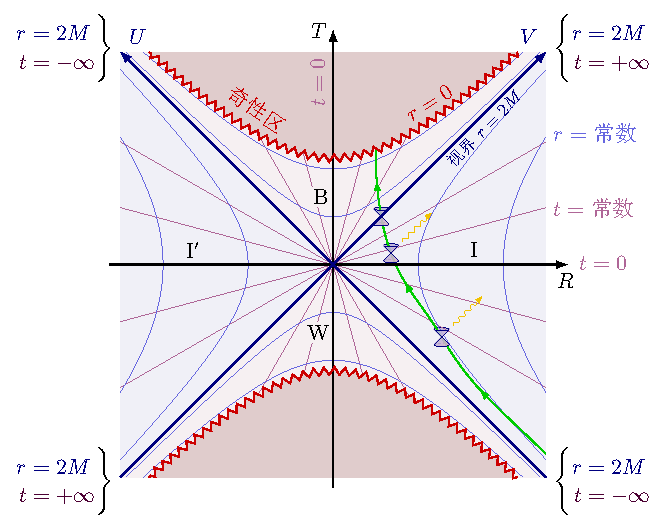
\includegraphics[width=15cm]{fig/II6-Kruskal.pdf}
    \caption{史瓦西度规的最大延拓:Kruskal--Szekeres坐标
        \protect\footnotemark[9] } \label{chsch:fig_Kruskal}
\end{figure}
{\footnotetext[9]{本图取自\url{https://tikz.net/relativity_kruskal_diagram/}.}}






图\ref{chsch:fig_Kruskal}描述了Kruskal--Szekeres坐标.
分成四个区域:$I$、$I'$、$B$、$W$.
锯齿线表示$r=0$,是奇点;由锯齿线包围的有颜色(浅褐色)区域以及锯齿线本身不属于时空.
史瓦西真空度规\eqref{chsch:eqn_Schw-metric}只是$I$区.
我们需要给出其它几个区的坐标表达式,为此先描述一下$r=2M$是怎样一个区域.

\paragraph{事件视界}\label{chsch:sec_event-horizon}
标注为$U$、$V$的坐标线是$r=2M$的时空区域,称为{\heiti 事件视界}(event horizon);
这是一个嵌入到四维时空的类光超曲面.
事件视界的物理内涵是指视界面内不会对视界面外产生任何影响,
或者说视界外观测者无法观测视界面内的任何信息.

在这个区域有$T=\pm R$;或者说可表示为$U=0$和$V=0$.
从度规\eqref{chsch:eqn_Kruskal-metric-light}可直接验证
切矢量$(\frac{\partial}{\partial U})^a$、$(\frac{\partial}{\partial V})^a$是类光的;
也可利用变换\eqref{chsch:eqn_RTUV}得到
\begin{equation*}
    \left(\frac{\partial}{\partial U}\right)^a = 
    \frac{1}{2} \left(\frac{\partial}{\partial T}\right)^a-
    \frac{1}{2} \left(\frac{\partial}{\partial R}\right)^a,\quad
    \left(\frac{\partial}{\partial V}\right)^a = 
    \frac{1}{2} \left(\frac{\partial}{\partial T}\right)^a+
    \frac{1}{2} \left(\frac{\partial}{\partial R}\right)^a.
\end{equation*}
然后利用度规\eqref{chsch:eqn_Kruskal-metric}验证
切矢量$(\frac{\partial}{\partial U})^a$、$(\frac{\partial}{\partial V})^a$是类光的.
超曲面$V=0$的法矢量是$(\frac{\partial}{\partial U})^a$,
超曲面$U=0$的法矢量是$(\frac{\partial}{\partial V})^a$;
这便证明了超曲面的类光性.

在$I$区,不难得到变换关系如下
\begin{equation}
    \left(\frac{r}{2M}-1\right) \exp{\frac{r}{2M}} = R^2-T^2= -U V;
    \quad \exp\frac{t}{2M}= -\frac{V}{U} .
\end{equation}
绿色类时线代表了有质量质点的运动轨迹,在$I$区,当此质点无限趋近于
超曲面$U=0^{-}$($V$坐标线)时,$r\to 2M^{+}$;因$I$区中$-\infty< U <0$、$0<V<+\infty $,
故由上式可知此时$t\to +\infty$.
同理,不难得到超曲面$V=0^{+}$($U$坐标线)上有$r\to 2M^{+}$、$t\to -\infty$.
\qed

不难发现在$I$区,有坐标变换关系:
\begin{equation}
    U= -\sqrt{\frac{r}{2M}-1}\, \exp\left(\frac{r-t}{4M}\right), \quad
    V= +\sqrt{\frac{r}{2M}-1}\, \exp\left(\frac{r+t}{4M}\right).
\end{equation}
根据因$I$区中的$-\infty< U <0$、$0<V<+\infty $;
在$B$区($0< U <+\infty$、$0<V<+\infty $,不含$r\leqslant 0$区域),我们将上述坐标变换关系延拓为:
\begin{equation}
    U= +\sqrt{1-\frac{r}{2M}}\, \exp\left(\frac{r-t}{4M}\right), \quad
    V= +\sqrt{1-\frac{r}{2M}}\, \exp\left(\frac{r+t}{4M}\right).
\end{equation}
$I'$($0< U <+\infty$、$-\infty< V <0$)是$I$的镜像区,故坐标变换延拓为
\begin{equation}
    U= +\sqrt{\frac{r}{2M}-1}\, \exp\left(\frac{r-t}{4M}\right), \quad
    V= -\sqrt{\frac{r}{2M}-1}\, \exp\left(\frac{r+t}{4M}\right).
\end{equation}
$W$($-\infty< U <0$、$-\infty< V <0$,不含$r\leqslant 0$区域)是$B$的镜像区,故有
\begin{equation}
    U= -\sqrt{1-\frac{r}{2M}}\, \exp\left(\frac{r-t}{4M}\right), \quad
    V= -\sqrt{1-\frac{r}{2M}}\, \exp\left(\frac{r+t}{4M}\right).
\end{equation}
由上述变换,不难得到下述变换:
\begin{align}
    &I\text{区}\ 
    \begin{cases}
       R = \sqrt{\frac{r}{2M}-1}\, \exp\left(\frac{r}{4M}\right)\, \cosh\left(\frac{t}{4M}\right) \\
       T = \sqrt{\frac{r}{2M}-1}\, \exp\left(\frac{r}{4M}\right)\, \sinh\left(\frac{t}{4M}\right) 
    \end{cases} \label{chsch:eqn_SK-I} \\
    &    B\text{区}\ 
    \begin{cases}
         R = \sqrt{1-\frac{r}{2M}}\,\exp\left(\frac{r}{4M}\right)\,\sinh\left(\frac{t}{4M}\right) \\
         T = \sqrt{1-\frac{r}{2M}}\,\exp\left(\frac{r}{4M}\right)\,\cosh\left(\frac{t}{4M}\right) 
    \end{cases} \label{chsch:eqn_SK-B} \\
    & I'\text{区}\ 
    \begin{cases}
       R = -\sqrt{\frac{r}{2M}-1}\,\exp\left(\frac{r}{4M}\right)\,\cosh\left(\frac{t}{4M}\right) \\
       T = -\sqrt{\frac{r}{2M}-1}\,\exp\left(\frac{r}{4M}\right)\,\sinh\left(\frac{t}{4M}\right) 
    \end{cases} \label{chsch:eqn_SK-Ip} \\
    &W\text{区}\ 
    \begin{cases}
       R = -\sqrt{1-\frac{r}{2M}}\,\exp\left(\frac{r}{4M}\right)\,\sinh\left(\frac{t}{4M}\right) \\
       T = -\sqrt{1-\frac{r}{2M}}\,\exp\left(\frac{r}{4M}\right)\,\cosh\left(\frac{t}{4M}\right) 
    \end{cases} \label{chsch:eqn_SK-W} 
\end{align}
以及逆变换
\begin{align}
&I,I',B,W \text{区}:\    \left(\frac{r}{2M}-1\right) \exp{\frac{r}{2M}} = R^2-T^2= -U V  .  \label{chsch:eqn_tr-TR}  \\
&I,I' \text{区}:\       \frac{t}{4M} = \tanh^{-1} \frac{R}{T};\qquad \exp\frac{t}{2M}= -\frac{V}{U} . \label{chsch:eqn_tr-VU-IIp} \\
&B,W \text{区}:\        \frac{t}{4M} = \coth^{-1} \frac{R}{T};\qquad \exp\frac{t}{2M}= +\frac{V}{U} . \label{chsch:eqn_tr-VU-BW}
\end{align}

在$B$区,当用逆变换将Kruskal--Szekeres度规变回史瓦西坐标$\{t,r,\theta,\phi\}$时,
线元表达式与史瓦西度规\eqref{chsch:eqn_Schw-metric}相同;请读者验证此点.
进而可验证,在$I'$、$W$区,史瓦西度规\eqref{chsch:eqn_Schw-metric}仍旧成立,
只不过在$r=2M$区域($U=0$、$V=0$)处无意义.
也就是说在史瓦西坐标$\{t,r,\theta,\phi\}$下,所有四个区的度规表达式是一样的,
但被分割成了四个不连通的区域.这正是坐标奇性的体现.


在$I$、$I'$区,由式\eqref{chsch:eqn_tr-VU-IIp}可知,当$t$是常数时,
$V/U$(或$X/T$)是常数;如图\ref{chsch:fig_Kruskal}所示.
同理,在$B$、$W$区,由式\eqref{chsch:eqn_tr-VU-BW}可得相同结论.

在四个区域,由式\eqref{chsch:eqn_tr-TR}可知,当$r$是常数时,
$U$、$V$(或$T$、$R$)构成双曲线;如图\ref{chsch:fig_Kruskal}所示,
而且图中的双曲线就是根据不同$r$值所绘.


\subsection{Killing矢量场}


很明显,每区都有与球对称的相对应的三个类空矢量场.

容易看出,在$I$区,$(\frac{\partial }{\partial t})^a$是类时Killing矢量场;
在$B$区,$(\frac{\partial }{\partial t})^a$是类空Killing矢量场(请读者验证之).
在$B$区的类时场是$(\frac{\partial }{\partial r})^a$,但它不是Killing矢量场;
因此$B$区不是定态的,更不可能是静态的.

由式\eqref{chsch:eqn_tr-VU-IIp}、\eqref{chsch:eqn_tr-VU-BW}可求得在$I$、$B$区
\begin{equation}\label{chsch:eqn_xi0}
    \left(\frac{\partial }{\partial t}\right)^a=
    \frac{ 1}{4 M } \left[-U \left(\frac{\partial }{\partial U}\right)^a
    +V \left(\frac{\partial }{\partial V}\right)^a \right] .
\end{equation}
因类光切矢量$(\frac{\partial }{\partial U})^a$、$(\frac{\partial }{\partial V})^a$在
事件视界区($r=2M$)是有定义的,故我们可以将$(\frac{\partial }{\partial t})^a$的
表达式\eqref{chsch:eqn_xi0}延拓至事件视界区.
容易验证在事件视界区($r=2M$),$(\frac{\partial }{\partial t})^a$是类光的.
还可以证明在事件视界区($r=2M$),$(\frac{\partial }{\partial t})^a$是Killing矢量场;
为此我们先给出事件视界区($r=2M$),$r$的几个导数:
\begin{align}
    \frac{\partial r}{\partial U}=& -V \exp\left(-\frac{r}{2M}\right) \frac{4M^2}{r},\quad
    \frac{\partial r}{\partial V}=  -U \exp\left(-\frac{r}{2M}\right) \frac{4M^2}{r}. %\\
%    \frac{\partial r}{\partial T}=& -T \exp\left(-\frac{r}{2M}\right) \frac{8M^2}{r},\quad
%    \frac{\partial r}{\partial R}=  +R \exp\left(-\frac{r}{2M}\right) \frac{8M^2}{r}.
\end{align}
在$\{U,V\}$坐标下,由度规\eqref{chsch:eqn_Kruskal-metric-light}求得非零克氏符为
\begin{equation*}
    \Gamma^U_{UU} = \frac{2M}{r}\left(1+\frac{2M}{r}\right) \exp\left(\frac{-r}{2M}\right) V,\quad
    \Gamma^V_{VV} = \frac{2M}{r}\left(1+\frac{2M}{r}\right) \exp\left(\frac{-r}{2M}\right) U.
\end{equation*}
可求得$\xi_a=g_{ab}(\frac{\partial }{\partial t})^b$协变导数的非零分量如下:
\begin{align*}
    \nabla_{\partial_U}\xi_U =& +\frac{2 M + r}{2 M r} UV \exp\left(-\frac{r}{2M}\right) \frac{4M^2}{r} -1 ,\\
    \nabla_{\partial_V}\xi_V =& -\frac{2 M + r}{2 M r} VU \exp\left(-\frac{r}{2M}\right) \frac{4M^2}{r} +1 .
\end{align*}
由上式可见,对与矢量场$\xi_a=g_{ab}(\frac{\partial }{\partial t})^b$有
$\nabla_a \xi_b+\nabla_b \xi_a=0$,也就证明了$\xi_a$是事件视界区($r=2M$)的Killing矢量场.

这样,Kruskal--Szekeres坐标系下共有四个Killing场,
与球对称相对应的三个是类空的;$(\frac{\partial }{\partial t})^a$在$r>2M$区类时,
在$r=2M$区类光,在$r<2M$区类空.


\subsection{Eddington--Finkelstein坐标系}

在Kruskal--Szekeres坐标中计算测地线较为复杂,很难积分出初等函数解.
我们介绍内向Eddington--Finkelstein坐标系来计算测地线;
这个坐标系不能覆盖图\ref{chsch:fig_Kruskal}中四个区域,但可以覆盖$I$和$B$区.

在式\eqref{chsch:eqn_tortoise}中,我们已经积分出乌龟坐标;
在式\eqref{chsch:eqn_uvtrs}引入了新的坐标$\{u,v\}$;
内向Eddington--Finkelstein坐标系取的参数是$\{v,r,\theta,\phi\}$,
即把史瓦西坐标中的$t$换成$v\equiv t+r_*$,其它三个坐标不换;
则史瓦西线元\eqref{chsch:eqn_Schw-metric}变为
\begin{equation}\label{chsch:eqn_EF-metric}
    {\rm d}s^2 = - \left(1-\frac{2 M}{r}\right) ({\rm d}v)^2
    + 2 {\rm d}r {\rm d}v + r^2 {\rm d}\Omega.
\end{equation}
很明显此时的度规在$r=2M$不是奇异的.
%算出非零克氏符
%\begin{subequations}\label{chsch:eqn_EF-Christoffel}
%    \begin{align}
%        &\Gamma^0_{00}= \frac{M}{r^2},\quad
%        \Gamma^0_{22}= -r,\quad
%        \Gamma^0_{33}= -r\sin^2\theta,\quad
%        \Gamma^1_{00}= \frac{M (r-2 M)}{r^3}, \\
%        &\Gamma^1_{01}=\Gamma^1_{10}= -\frac{M}{r^2}, \quad
%        \Gamma^1_{22}= 2 M-r, \quad
%        \Gamma^1_{33}= (2 M-r) \sin ^2\theta  , \\
%        &\Gamma^2_{12}=\Gamma^2_{21}= \frac{1}{r}, \quad
%        \Gamma^2_{33}=-\sin\theta \cos\theta, \quad
%        \Gamma^3_{13}=\Gamma^3_{31}=\frac{1}{r}, \quad
%        \Gamma^3_{23}=\Gamma^3_{32}=\cot\theta . \notag
%    \end{align}
%\end{subequations}
%只涉及$\theta$、$\phi$指标的克氏符与史瓦西坐标下的克氏符相同.


度规\eqref{chsch:eqn_EF-metric}中的参数$-\infty<v<+\infty$对应Kruskal--Szekeres坐标中$0<V<+\infty$;
故内向Eddington--Finkelstein坐标系能覆盖图\ref{chsch:fig_Kruskal}中$I$和$B$区.
度规\eqref{chsch:eqn_EF-metric}中的系数不含有坐标$v$,
故$(\frac{\partial}{\partial v})^a$是Killing场,
容易可验证在$I$区它是类时的,在$B$区是类空的.
由于$g_{rr}=0$,故$(\frac{\partial}{\partial r})^a$是类光的.


设有类时曲线$\gamma(\tau)$,$\tau$是固有时,曲线参数化为$(v,r,\pi/2,\phi)$,
其切线切矢量指向未来(见图\ref{chsch:fig_Kruskal}中绿色线).
对于度规\eqref{chsch:eqn_EF-metric}来说,有
\begin{equation}\label{chsch:eqn_tmp-tl}
    g_{ab}\left(\frac{\partial}{\partial \tau}\right)^a \left(\frac{\partial}{\partial \tau}\right)^b
    = - \left(1-\frac{2 M}{r}\right) \dot{v}^2 + 2 \dot{v} \dot{r} + r^2 \dot{\phi}^2 = -1 < 0
\end{equation}
上式中的“点”表示对$\tau$求导数.因$r^2 \dot{\phi}^2$非负,故由上式可得
\begin{equation}
    \dot{v}\left[- \left(1-\frac{2 M}{r}\right) \dot{v} + 2  \dot{r}\right]  < 0.
\end{equation}
在$I$区,$v$是坐标时,因$\gamma$是指向未来的,故有$\dot{v}>0$.
又因类时线$\gamma$本身连续、光滑,导数也是连续的;
故当$\gamma$穿过$r=2M$区域进入$B$区时,$\dot{v}>0$也是成立的.
所以由上式可以得到在整条$\gamma$线上,有
\begin{equation}\label{chsch:eqn_tmp-rt}
    - \left(1-\frac{2 M}{r}\right) \dot{v} + 2  \dot{r} < 0.
\end{equation}
当$r>2M$时,随着$\tau$的增加,图\ref{chsch:fig_Kruskal}中绿色类时线$r$是逐渐减小的.
当$r\leqslant 2M$时,由\eqref{chsch:eqn_tmp-rt}可知其
第一项是非负的,故在$B$区类时线$\gamma(\tau)$上$\dot{r}<0$.
这样便说明了:不论$I$区还是$B$区,在整条绿色类时线$\gamma(\tau)$上,都有$\dot{r}<0$.
至此,我们证明了指向未来的类时线只能从$I$区穿越视界区($r=2M$),
然后进入$B$区;不能从$B$返回$I$区.
对于指向未来的绿色类时线而言(见图\ref{chsch:fig_Kruskal}),视界($r=2M$)是
一个{\kaishu 单向膜};正因为此,我们称$B$区为{\heiti 黑洞}.
那么它的镜像区$W$自然称为{\heiti 白洞}.
$I$和$B$区是相互连通的.
$I$和$I'$区是不因果连通,即没有类时线或类光线连接两个区域;
它们是两个全同的宇宙.

宇宙飞船的轨迹自然是指向未来的类时线,在飞船穿越$r=2M$之前,如果它开足马力返航,
是可以让$r$随$\tau$的增大而增大的,即$\dot{r}>0$;
可见图\ref{chsch:fig_Kruskal}中绿色类时线上的光锥.
但只要越过视界,便再也没有返航机会.


如果$\gamma$是类光线,$\tau$是一仿射参数.此时式\eqref{chsch:eqn_tmp-tl}中
右端不是等于“$-1$”,而是等于零.为简单起见,我们零$\dot{\phi}=0$,那么有
\begin{equation}
    - \left(1-\frac{2 M}{r}\right) \dot{v}^2 + 2 \dot{v} \dot{r} =0 .
\end{equation}
这说明类光线分为两组,即
\begin{equation}
    \frac{{\rm d}v}{{\rm d}\tau} =0, \quad \text{和}\quad 
    \frac{{\rm d}v}{{\rm d}r} = \frac{2r}{r-2M}.
\end{equation}
第一组只是相互平行的类光线,并无特别之处;略.
第二组类光线,当$r=2M$时,导数是无穷大,相当于在$v-r$图中的一条竖直向上的直线;
这是容易想象的:$r$是横轴,$v$是纵轴,在$r=2M$处,此线垂直于横轴、平行于纵轴.
当$r>2M$时($I$区),随着$r$的增大$v$是增大的.
当$r<2M$时($B$区),$v$是$r$的减函数;这说明在$B$区即便类光线也无法穿越视界返回$I$区.








\section{史瓦西解的NP型式描述}

\section{真空解唯一性定理}

真空爱因斯坦引力场方程的解唯一性定理不止一个,它们有重叠部分,也有不同部分.
我们叙述两个定理;更多、更新内容请参考综述文献\parencite{Chrusciel-2012-lrr}.

\subsection{Birkhoff定理}
\index[physwords]{Birkhoff定理}  

{\bfseries \heiti Birkhoff定理}:真空爱因斯坦场方程的球对称解必是史瓦西度规.%\cite[附录B]{hawking-ellis1973}

下面开始证明.球对称时空的度规
是\eqref{chhss_eqn_g-st-sphere}(${\rm d}\Omega\equiv({\rm d}\theta)^2 + (\sin\theta {\rm d}\phi)^2 $):
\begin{equation}
    \mathrm{d} s^2=  g_{t t}(r, t) \mathrm{d} t^2+2 g_{r t}(r, t) \mathrm{d} r \mathrm{d} t+g_{r r}(r, t) \mathrm{d} r^2 
    +r^2\mathrm{d} \Omega .    \tag{\ref{chhss_eqn_g-st-sphere}}
\end{equation}
由于此处未引入超曲面正交的前提条件,我们采用变换方式将$g_{r t}(r, t)$消掉.
只需定义一个新的{\kaishu 时间}$\tilde{t}$使得
\begin{equation}
    {\rm d}\tilde{t} = \chi(r,t) \bigl(g_{t t}(r, t) \mathrm{d} t+ g_{r t}(r, t) \mathrm{d} r \bigr),
\end{equation}
上式中$\chi$是积分因子,它使得上式右端是全微分;
这样的积分因子总是存在的,证明可参考\parencite[p. 387]{chenwh2017}定理1.2或类似文献.
则上述线元变为:
\begin{equation}
    \mathrm{d} s^2=  g_{t t}^{-1} \chi^{-2} \mathrm{d} \tilde{t}^2+
    \bigl(g_{r r}- g_{t t}^{-1} g_{rt}^{2} \bigr)\mathrm{d} r^2 
    +r^2\mathrm{d} \Omega .
\end{equation}
为了使公式简单,我们引入新函数$\alpha(r,t)= g_{t t}^{-1} \chi^{-2}$、
$\beta(r,t)=g_{r r}- g_{t t}^{-1} g_{rt}^{2}$,并将$\tilde{t}$简记为$t$;
则上述线元变为:
\begin{equation}\label{chsch:eqn_timpshc0}
    \mathrm{d} s^2=  \alpha(r,t) \mathrm{d} t^2+
    \beta(r,t)\mathrm{d} r^2 +r^2\mathrm{d} \Omega .
\end{equation}
利用符号演算软件,由上述度规可得非零Ricci曲率:
\begin{align}
    R_{00} =& \frac{r \beta  ({\alpha'}^2+\dot{\alpha}  \dot{\beta} )
        +\alpha  \left(r (\dot{\beta} ^2+\alpha' \beta')
        -2 \beta  (2 \alpha'+r (\alpha''
        +\ddot{\beta} ))\right)}{4 r \alpha  \beta^2},\\
    R_{01} =& \frac{\dot{\beta} }{r \beta }, \label{chsch:eqn_Rtr}\\
    R_{11} =& \frac{\alpha  \left(4 \alpha  \beta'+r (\dot{\beta} ^2
        +\alpha' \beta')\right)+r \beta  \left(\alpha'^2
        +\dot{\alpha} \dot{\beta} -2 \alpha  (\alpha''
        +\ddot{\beta} )\right)}{4 r \alpha ^2 \beta },\\
    R_{22} =& \frac{1}{2} \left(-\frac{\frac{r \alpha'}{\alpha }+2}{\beta }
    +\frac{r \beta'}{\beta ^2}+2\right),\\
    R_{33} =& \frac{\sin ^2 \theta  \left(\alpha  \left(2 \beta ^2-2 \beta 
        +r \beta'\right)-r \beta  \alpha'\right)}{2 \alpha  \beta ^2} .
\end{align}
上式中“撇号”代表对$r$求导数,“点”代表对$t$求导数.
由于系数含时间$t$,故此处的引力场未必是定态的(或静态).
真空爱氏场方程为$R_{\mu\nu}=0$;
由式\eqref{chsch:eqn_Rtr}可知:$\beta$与时间无关.
从上述$R_{\mu\nu}$表达式容易看出所有与时间有关的导数都去掉了.
则上述真空引力场方程变为($R_{00}$、$R_{11}$、$R_{22}$):
\begin{align}
    0 =& r \beta  {\alpha'}^2  + r \alpha \alpha' \beta'
          -4 \alpha \beta  \alpha'-2 r\alpha \beta  \alpha'' ,\label{chsch:eqn_tmp-r00}\\
    0 =& r \beta \alpha'^2+r  \alpha \alpha' \beta'
    +   4 \alpha^2 \beta'   -2 r\alpha \beta \alpha'' ,\label{chsch:eqn_tmp-r11}\\
    0 =& 2 \alpha\beta ^2-2\alpha \beta +r\alpha \beta'-r \beta  \alpha' . \label{chsch:eqn_tmp-r22}
\end{align}
式\eqref{chsch:eqn_tmp-r11}减去\eqref{chsch:eqn_tmp-r00}得
\begin{equation}\label{chsch:eqn_abp0}
    0= \alpha \beta' + \beta  \alpha' = (\alpha \beta)' .
\end{equation}
由上式得$\alpha'=-\alpha \beta'/\beta$,带入式\eqref{chsch:eqn_tmp-r22}并整理得
\begin{equation}
    \left(\frac{r}{\beta}\right)'=1 .
\end{equation}
因$\beta$与时间无关,故由上两式可得(已将积分常数取得与史瓦西度规相同):
\begin{equation}
    \alpha=- f(t) \left(1- \frac{2M}{r}\right),\qquad
    \beta= \left(1- \frac{2M}{r}\right)^{-1}.
\end{equation}
上式中$f(t)$是恒正函数.定义新的时间坐标$t'$:
\begin{equation}
    t'\equiv \int_{}^{t} \sqrt{f(p)} {\rm d}p .
\end{equation}
这样,线元\eqref{chsch:eqn_timpshc0}变为
\begin{equation}
    \mathrm{d} s^2=  - \left(1- \frac{2M}{r}\right)\mathrm{d} t'^2+
    \left(1- \frac{2M}{r}\right)^{-1}\mathrm{d} r^2 +r^2\mathrm{d} \Omega .
\end{equation}
最后,线元与史瓦西度规\eqref{chsch:eqn_Schw-metric}完全相同.

需要强调的是:当$r<2M$时,$t$是类空坐标线,$r$是类时坐标线.
此时度规场并非定态.
在证明Birkhoff定理过程中,我们没有假设存在类时Killing矢量场,
只假设了时空是球对称的(包含三个类空Killing场).
通过求解爱氏引力场方程,我们得到了第四个Killing场$(\frac{\partial}{\partial t})^a$,
它可能类时($r>2M$),可能类空($r<2M$),可能类光($r=2M$).


\subsection{Israel定理}
\index[physwords]{Israel定理}

\subsubsection{曲率表述等}
下面给出Israel定理的证明\cite{Israel-1967}. %\cite{Robinson-1977}
由于$M$是四维静态时空,故存在与类空超曲面$\Sigma_t$正交的类时Killing矢量
场$\xi^a=(\frac{\partial }{\partial t})^a$;故度规可以写成:
\begin{equation}
    \mathrm{d} s^2=  -N^2 \mathrm{d} t^2+g_{ij} \mathrm{d} x^i  \mathrm{d} x^j.
\end{equation}
$N(>0)$、$g_{ij}$均是空间坐标$\{x^i\}$的函数,不含有时间$t$.
$g_{ij}$是类空超曲面$\Sigma_t$上的度规.
容易算出非零的克氏符$\Gamma^{0}_{\mu\nu}$为
\begin{align}
    \Gamma^{0}_{01}=\Gamma^{0}_{10}= \frac{\partial_{x^1}N}{N},\quad
    \Gamma^{0}_{02}=\Gamma^{0}_{20}= \frac{\partial_{x^2}N}{N},\quad
    \Gamma^{0}_{03}=\Gamma^{0}_{30}= \frac{\partial_{x^3}N}{N}.
\end{align}
当度规的$g_{0i}=0$且各个分量不含时间$t$的时候,曲率公式还能进一步简化.
由于超曲面正交,故ADM分解(见\S\ref{chsm:sec_ADM})后的
位移矢量场$S^a=0$;则有
\begin{equation}
    \left(\frac{\partial }{\partial t}\right)^a = N n^a ;\qquad
    ({\rm d}t)_a = -\frac{1}{N} n_a .
\end{equation}
由外曲率公式\eqref{chsm:eqn_Kab-1}或\eqref{chsm:eqn_K-Christoffel}计算可以得到$K_{ab}=0$;
或者,因度规分量不含时且$S^a=0$,由公式\eqref{chsm:eqn_Lie-t-hab}同样
可得类空超曲面$\Sigma_t$上的外曲率恒为零.
外曲率为零给超曲面上黎曼曲率、Ricci曲率的计算带来诸多方便.
由式\eqref{chsm:eqn_tmp-c0}可知
\begin{equation}\label{chsch:eqn_R4i0}
    {}^{4}{R}_{0i} =0 ,\qquad 1 \leqslant i \leqslant 3 .
\end{equation}
再由式\eqref{chsm:eqn_contractRicci}可得
\begin{equation*} %\label{chsch:eqn_tmp-Rik}
    {}^{3}{R}_{ik}  ={}^{4} {R}_{ik} + {}^{4}{R}_{i0k0}  N^{-2} .
\end{equation*}
经计算有$\Gamma_{0k}^l=0$($1 \leqslant k,l \leqslant 3$).
我们用式\eqref{chrg:eqn_Riemannian04-component}来计算${}^{4}{R}_{i0k0}$:
\begin{align*}
    {}^{4}R_{i0k0} =& -\frac{1}{2}
    \frac{\partial^2 g_{00}} {\partial x^i\partial x^k}
    + g_{00}\Gamma_{0k}^0\Gamma_{0i}^0
    + g_{lp}\left( \Gamma_{0k}^l\Gamma_{0i}^p - \Gamma _{00}^l\Gamma_{ik}^p \right) \\
%    =& N\frac{\partial^2 N} {\partial x^i\partial x^k}
%    +\frac{\partial N} {\partial x^i}\frac{\partial N} {\partial x^k}
%    -\frac{\partial N} {\partial x^i}\frac{\partial N} {\partial x^k}
%    - g_{lp} \Gamma _{00}^l\Gamma_{ik}^p \\
    =& N\frac{\partial^2 N} {\partial x^i\partial x^k}
    -  N \frac{\partial N}{\partial x^p}  \Gamma_{ik}^p 
    = N \nabla_i \nabla_k N .
\end{align*}
带回上上式,有
\begin{equation}\label{chsch:eqn_R4ij}
    {}^{4}{R}_{ik}  ={}^{3} {R}_{ik} -  N^{-1} \nabla_i \nabla_k N .
\end{equation}
下面计算${}^{4}R_{00}$.由式\eqref{chsm:eqn_contractR}可知:
$ {}^{3}{R}={}^{4}{R}+ {}^{4}{R}_{00}  N^{-2} \times 2 $.
而
$    {}^{4}{R} =  {}^{4}R_{\rho\sigma} g^{\rho\sigma}
    = {}^{4}R_{00} g^{00} +  {}^{4}R_{ik}g^{ik}
    \xlongequal{\ref{chsch:eqn_R4ij}} - {}^{4} R_{00}N^{-2} 
    + {}^{3} {R}_{ik} g^{ik} -  N^{-1} g^{ik} \nabla_i \nabla_k N $.
带回,有
\begin{equation}\label{chsch:eqn_R400}
    {}^{4}{R}_{00}  =   N g^{ik} \nabla_i \nabla_k N ;    \quad\text{及}\quad
    {}^{4}{R}={}^{3}{R} - 2N^{-1}g^{ik} \nabla_i \nabla_k  N  .
\end{equation}
由式\eqref{chsch:eqn_R4i0}、\eqref{chsch:eqn_R4ij}、\eqref{chsch:eqn_R400}可以
得到真空爱因斯坦场方程(${}^{4}R_{\mu\nu}=0$).
%由式\eqref{chsch:eqn_R4i0}恒为零和$g_{0i}=0$,可知${}^{4}{G}_{0i}\equiv 0$;
%继而,不难得到
%\begin{equation}\label{chsch:eqn_G4}
%\begin{aligned}
%    {}^{4}{G}_{00} &
%    %={}^{4}{R}_{00} - {}^{4}{R} \frac{1}{2} g_{00}
%    %=N g^{ik} \nabla_i \nabla_k N  +\frac{N^2}{2} ({}^{3}{R} - 2N^{-1}g^{ik} \nabla_i \nabla_k )
%    ={}^{3}{R} \times \frac{N^2}{2}; 
%    \qquad {}^{4}{G}_{0i}\equiv 0; \\
%    {}^{4}{G}_{ij}&
%    %={}^{4}{R}_{ij} - {}^{4}{R} \frac{1}{2} g_{ij}
%    %={}^{3} {R}_{ij} -  N^{-1} \nabla_i \nabla_j N 
%    %-\frac{g_{ij}}{2} ({}^{3}{R} - 2N^{-1}g^{kl} \nabla_l \nabla_k N)
%    ={}^{3}{G}_{ij} - N^{-1} \left( \nabla_i \nabla_j N - g_{ij} (g^{kl} \nabla_k \nabla_l N)\right).
%\end{aligned}
%\end{equation}

%我们已用参数$t$将时空$M$分解为$\mathbb{R}\times \Sigma_t$;下面,进一步分解$\Sigma_t$.
%现在我们采取一个技术性假设\cite{Israel-1967}:可以利用$N$等于常数进一步
%将三维类空超曲面$\Sigma_t$分解为一系列二维曲面,这一过程称为{\kaishu 叶化}(Foliation).
%这样$\Sigma_t$上的线元简化为(我们将四维线元$\mathrm{d} s^2$记
%为$\mathrm{d} s^2=-N^2 \mathrm{d} t^2+{\rm d}\hat{s}^2$):
%\begin{equation}\label{chsch:eqn_S2metric}
%    {\rm d}\hat{s}^2 = \sum_{i,j=1}^{3} g_{ij} \mathrm{d} x^i  \mathrm{d} x^j
%    = \rho^2 {\rm d}N^2 + \sum_{A,B=2}^{3}\hat{g}_{AB}\mathrm{d} x^A  \mathrm{d} x^B.
%\end{equation}
%在本节剩余部分,我们约定大写拉丁字母($A$、$B$等)求和范围是:$2$、$3$.
%为简单起见,我们将第一个坐标记为:$x^1\equiv N$.
%至此,我们将三个类空坐标的第一个分离出来.
%需要再次强调一下,$\rho$、$\hat{g}_{AB}$是$x^1\equiv N$、$x^2$、$x^3$的函数场.
%
%虽然三维类空超曲面$\Sigma_t$的外曲率为零,但通过上述方式叶化后的二维曲面的外曲率不是零.
%通过式\eqref{chsm:eqn_K-Christoffel}可得
%\begin{equation}
%    K_{AB} = {n}_a \Gamma_{AB}^a(\hat{g}) = \rho \Gamma_{AB}^1(\hat{g}) 
%    = - \frac{1}{2\rho}  \frac{\partial \hat{g}_{AB}}{\partial x^1} .
%\end{equation}
%
%由式\eqref{chsch:eqn_S2metric}中$\hat{g}_{AB}$描述的二维曲面来说,
%\begin{equation}
%    \left(\frac{\partial }{\partial N}\right)^a = \rho n^a ;\qquad
%    ({\rm d}N)_a = \frac{1}{\rho} n_a .
%\end{equation}
%再由式\eqref{chsm:eqn_G-Gauss}、\eqref{chsm:eqn_G-Codazzi}得如下式子
%\begin{align}
%    {}^{3}G_{11} \rho^{-2} =& {}^{3}G_{ab} {n}^{a} {n}^{b}    
%    ={}^{2}{R}\frac{-1}{2}   + \frac{1}{2} (K^2 - K^{AB} K_{AB} )  . \\
%    {}^{3}G_{1A} \rho^{-1} =& {}^{3}G_{ab}{n}^{a} h^{b}_A
%    = {\rm D}_A K -{\rm D}_B K_{A}^B ; \quad\text{其中}\
%    K = \hat{g}^{AB}K_{AB}.
%\end{align}


\subsubsection{定理证明}

由$\xi^b$是与超曲面$\Sigma$正交的类时Killing矢量场可知$g_{ab}\xi^a \xi^b = -N^2$;有
\begin{equation}\label{chsch:eqn_Dxi}
    -N\nabla_a N= \xi^b \nabla_a \xi_b = -\xi^b \nabla_b \xi_a .
\end{equation}
我们计算两个式子.
\begin{align*}
    (\nabla_a \xi_b) \nabla^a \xi^b =& \nabla_a \left( \xi_b \nabla^a \xi^b\right)
    -\xi_b \nabla_a \nabla^a \xi^b
    \xlongequal[\ref{chrg:eqn_killing-Riemann-2}]{\ref{chsch:eqn_Dxi}}
    - \nabla^a (N\nabla_a N ) + \xi^b R_{eb}{\xi^e} . \\
    (\nabla_b \xi_a) \nabla^a \xi^b =& \nabla_b \left( \xi_a \nabla^a \xi^b\right)
    -\xi_a \nabla_b \nabla^a \xi^b
    \xlongequal[\ref{chrg:eqn_killing-Riemann-1}]{\ref{chsch:eqn_Dxi}}
    + \nabla^b (N\nabla_b N ) - \xi^a R_{a}^e{\xi_e} .
\end{align*}
考虑到真空爱氏场方程为$R_{ae}=0$,以及$N$是谐和的(式\eqref{chsch:eqn_R400}),有
\begin{equation}\label{chsch:eqn_Wxi}
    \rho \overset{def}{=} -  (\nabla_{[a} \xi_{b]}) \nabla^a \xi^b
    %    = \frac{1}{2}(\nabla_b \xi_a-\nabla_a \xi_b) \nabla^a \xi^b
    %    = \nabla^b (N\nabla_b N )
    =g^{ik}(\nabla_i N) \nabla_k N .
\end{equation}
故$\rho$是正的.



定义
\begin{equation}
    {}^{3}R_{ijk}\overset{def}{=} {}^{3}R_{ij;k}- \frac{1}{4}g_{ij}\times {}^{3}R_{;k}
    -{}^{3}R_{ik;j}+ \frac{1}{4}g_{ik}\times {}^{3}R_{;j} .
\end{equation}
由真空爱氏场方程可知${}^{4}{R}=0$(请注意四维、三维的差别);
再由\eqref{chsch:eqn_R400}式的后半部分可知:
${}^{3}{R} = 2N^{-1}g^{ij} \nabla_i \nabla_j N $.
真空爱氏场方程还要求${}^{4}{R}_{00}  = 0$;
再由\eqref{chsch:eqn_R400}式的前半部分可知:${}^{3}{R} =0$.
那么自然有${}^{3}{R}_{;k}=0$.
继而,由式\eqref{chsch:eqn_R4ij}可知(爱氏场方程${}^{4}{R}_{ik}=0$):
${}^{3} {R}_{ik} =  N^{-1} \nabla_i \nabla_k N $.
计算
\setlength{\mathindent}{0em}
\begin{align*}
    &{}^{3}R_{ijk} \  {}^{3}R^{ijk}= \nabla_k (N^{-1} \nabla_j \nabla_i N)
    \nabla^k (N^{-1} \nabla^j \nabla^i N) \\
    =&\left(-N^{-2}(\nabla_k N)\nabla_j \nabla_i N + N^{-1} \nabla_k  \nabla_j \nabla_i N \right)
    \left(-N^{-2}(\nabla^k N)\nabla^j \nabla^i N + N^{-1} \nabla^k  \nabla^j \nabla^i N \right)\\
    =& +N^{-4}(\nabla_k N)(\nabla_j \nabla_i N )(\nabla^k N)\nabla^j \nabla^i N
    + N^{-2} ( \nabla_k  \nabla_j \nabla_i N)\nabla^k  \nabla^j \nabla^i N \\
    &- N^{-3}(\nabla_k N)(\nabla_j \nabla_i N)\nabla^k  \nabla^j \nabla^i N
    - N^{-3} ( \nabla_k  \nabla_j \nabla_i N)(\nabla^k N)\nabla^j \nabla^i N     \\
    =&
\end{align*}\setlength{\mathindent}{2em}

\begin{align*}
    c=& 4N^{-4} \rho \nabla^i \nabla_i \rho- 4N^{-5} \rho \nabla^i \rho \nabla_i N - 3 N^{-4} \nabla^i\rho \nabla_i \rho \\
    =& + 4N^{-4} (\nabla^k N \nabla_k N) \nabla^i \nabla_i(\nabla^j N \nabla_j N) \\
    &- 4N^{-5} (\nabla^k N \nabla_k N) \nabla^i (\nabla^j N \nabla_j N) \nabla_i N \\
    &- 3 N^{-4} \nabla^i(\nabla^k N \nabla_k N) \nabla_i (\nabla^j N \nabla_j N) \\
    =&
\end{align*}

{\bfseries \heiti Israel定理}:
广义相对论中,静态、真空引力场必是球对称的,
由史瓦西度规描述.史瓦西度规是唯一静态真空引力场.

\section*{小结}
本章主要参考了\parencite[Ch.3]{chandrasekhar-1983}、\parencite{mtw1973}相应章节.

%%%%%%%%%%%%%%%%%%%%%%%%%%%%%%%%%%%%%%%%%%%%%%%%%%%%%%%%%%%%%%%%%%%%%%%%%%%%%%%%%%%
\printbibliography[heading=subbibliography,title=第\ref{chsch}章参考文献]

\endinput
